\begin{document}
	\chapter{Implementation}
	This chapter describes the describes how the requirements described in the previous chapter have been accomplished. 
	\section{Overall structure of the project} \label{Section: impl/overview}
	The main objective I had while implementing the project was to be able to have a completely independent tool that is can communicate with the CADETS client and classify nodes successfully. In order to achieve this, I divided the overall project into three smaller sub-modules:
	
	\begin{enumerate}
		\item \label{impl/overview/enum/1} The \textbf{Neo4J interface}, which handles the interaction between my tool and the Neo4J database that stores the raw graph data with the end purpose of extracting the nodes' feature vectors. This is described in detail in Section \ref{Section: impl/neo4j}.
		\item The \textbf{machine learning models}, which use the feature vectors extracted as part of the \ref{impl/overview/enum/1}$^{\text{st}}$ module in order to classify the nodes into \textit{SHOW} or \textit{HIDE}. The exact details of how they were implemented in Section \ref{Section: impl/ml}.
		\item The \textbf{REST API}, which wraps around the previous two modules and handles requests received by the tool. This is described in detail in Section \ref{Section: impl/REST}.
	\end{enumerate}
	Figure \ref{Fig: impl/pipeline} shows a schema of how the 3 modules will work together as a part of a request processing pipeline. 
	\\ \\
	In the following sections, I will describe the modules listed above in a bottom-up approach -- from the Neo4J interaction to the REST API. 
	\begin{figure}[H]
		\centering
		\includegraphics[width=.95\textwidth]{graphics/overall-schema}	
		\caption[Processing pipeline]{Overview of the project's processing pipeline.}
		\label{Fig: impl/pipeline}
	\end{figure}
	\section{Neo4J interaction} \label{Section: impl/neo4j}
	This section describes how the project I implemented interacts with the Neo4J database and how the features for every node are extracted. 
	\subsection{Database driver} \label{Section: impl/neo4j/driver}
	The biggest challenge when designing the database driver was the choice of the library I would use to run the actual queries. There are a number of Python libraries available, out of which I took two into consideration: \textbf{py2neo}\footnote{\textbf{\url{http://py2neo.org/v3/}}} and \textbf{neo4j-driver}\footnote{\textbf{\url{https://github.com/neo4j/neo4j-python-driver}}}. In order to decide which one I will use, I timed the running of two queries(\textit{match (n) return n} and \textit{match(n) return n limit 1} ) and the overall feature extraction for one node on a database of $631, 357 \text{ nodes}$ for both libraries. The resulting times are shown in Table \ref{Table: impl/neo4j-driver-timings}:
	\begin{longtable}{|p{.15\textwidth}|p{.30\textwidth}p{.25\textwidth}p{.25\textwidth}|}
		\textbf{library} & \textbf{\textit{match(n) return n}} & \textbf{\textit{match(n) return n limit 1}} & \textbf{feature extraction} \\
		\hline
		\textit{py2neo} & $337.477\text{s } (\approx5.5 \text{ minutes})$ & $13\text{ms}$ & TODO \\ 
		\textit{neo4j-driver} & $97.288\text{s }(\approx1.5 \text{ minutes})$ & $28\text{ms}$ & $68.78\text{s}$  \\
		\hline
		\caption[Neo4J libraries timings]{\centering Table showing the timings for the two libraries considered}
		\label{Table: impl/neo4j-driver-timings}
	\end{longtable}
	The main purpose of the database driver is to support feature extraction(detailed in Section \ref{Section: impl/neo4j/features}). Therefore, given the times in Table \ref{Table: impl/neo4j-driver-timings}, I decided to use \textbf{neo4j-driver}. On top of this library, I wrote a wrapper class, \textbf{DatabaseDriver}. 
	\subsection{Feature extractor} \label{Section: impl/neo4j/features}
	The feature extractor uses the DatabaseDriver described in the previous section in order to build the feature vectors for a list of nodes, just as described in Table \ref{Table: prep/features}. Therefore, the two classes will be in an association relationship (i.e. the FeatureExtractor has one instance of DatabaseDriver), as displayed in Figure \ref{Fig: impl/neo4j-driver-uml}.
	\\ \\
	Considering the fact that the machine learning models require purely real feature vectors to work, I decided to use \textbf{onehot-hot-encoding} for the categorical features. In other words, for every such feature, I generated one extra boolean column for each category. Only one of these columns can take the value 1 for each sample. Using this encoding led to an increase in the length of the feature vectors, from 13 to 23 variables. 
	\\ \\
	On top of extracting the feature matrix, this module also has support for generating the adjacency matrix of the nodes from the list provided. This is required for models such as the Graph Attention Networks (Section \ref{Section: impl/ml/gat}).
	\begin{figure}[H]
		\centering
		\includegraphics[width=.5\textwidth]{graphics/umls/uml-neo4j-driver}
		\caption[FeatureExtractor UML class diagram]{\centering UML class diagram showing the interaction between the feature extractor and the database driver.}
		\label{Fig: impl/neo4j-driver-uml}
	\end{figure}
	\section{Machine learning module} \label{Section: impl/ml}
	With the first module being implemented, I started to implement different machine learning models that I would use to classify the nodes. 
	\subsection{Training set} \label{Section: impl/ml/training-set}
	One of the key requirements for a well-behaved machine learning model is to have a comprehensive training set. Keeping this in mind, I used the ground-truths listed in Section \ref{Section: prep/data/ground-truths} with the aim of extracting examples of nodes from both classes (i.e. \textit{SHOW} and \textit{HIDE}) from a database of $6,007$ nodes, out of which $5,498$ are of interest (i.e. either \textit{File}, \textit{Process} or \textit{Socket}). For all these selected nodes, I used the feature extractor in order to build a labelled training set $\mathbf{s}=\{ (\mathbf{x}_1, \mathbf{y_1}), \dots, (\mathbf{x}_n, \mathbf{y_n}) \}$ that will be used by all the models in the training phase. As expected, there is a significant imbalance in the training data, with $2,382$ nodes ($43.33\%$) being labelled as \textit{SHOW} and $3,115$ ($56.67\%$) being labelled as \textit{HIDE}. This is a factor that I took into consideration both when designing and evaluating the models.
	\\ \\
	Moreover, using the same training set for all the models implemented is one of the key factors that ensure the correctness of the models' comparative evaluation. 
	\subsection{The Keras ecosystem} \label{Section: impl/ml/ecosys}
	Keras is a high-level deep-learning API, that can run on top of TensorFlow\footnote{\textbf{\url{https://www.tensorflow.org/}}}, CNTK\footnote{\textbf{\url{https://github.com/Microsoft/cntk}}} or Theano\footnote{\textbf{\url{https://github.com/Theano/Theano}}}, providing user friendliness, modularity and extensibility. Therefore, it allows for easy and fast prototyping, fitting well with the software engineering approach I took during the implementation stage. Moreover, Keras modules are highly portable: a model developed using one backend can just as easily work on any other deep learning backend. For the implementation of the parametric techniques I experimented as part of this project, I used the TensorFlow backend for Keras. 
	\\ \\
	The core data structure of Keras is a \textbf{Model}, an abstraction that gives users the ability to organize different type of layers. For most of the models presented here, I used the \textbf{Sequential} model, which represents a linear stack of layers. Running a model in Keras consists of 4 core elements:
	\begin{enumerate}
		\item \textbf{definition} - initialising the model and using the \textit{.add()} method to add layers.
		\item \textbf{compilation} - using the \textit{.compile()} method to define the loss function and optimizer that the model will use during the training phase, as well as any hyperparameters that they require. At this stage, one can also define the metrics that will be for evaluating the model. 
		\item \textbf{training} - once the model was compiled, the \textit{.train()} method can be used to define the training and validation sets used for optimizing the weights and hyperparameters of the model, respectively. Here, the user can also define two other hyperparameters: the number of iterations for which the optimizer will run and the batch size, for batch-based methods. 
		\item \textbf{running} - with the model being optimized, the user can either use it to make predictions or to evaluate it, using the metrics defined in the compile stage. 
	\end{enumerate}
	\subsection{Regularization techniques} \label{Section: impl/ml/reg}
	When training neural networks, one of the most frequent problems that can occur is \textbf{overfitting}: the model fits corresponds too closely to the training data and therefore fails to generalize as expected. This section addresses the techniques that I applied in order to avoid overfitting and also to speed up the training phase of my models.  
	\subsubsection{Batch normalization} \label{Section: impl/ml/reg/batch}
	During the training phase, the distribution of each layer's input changes, as the parameters of the previous layer change, phenomenon known as \textit{internal covariance}. This slows down the training by requiring lower learning rates and careful parameter initialisation. 
	\\ \\
	In this section, I describe one technique for addressing this problem, by normalizing layer inputs. This technique is known as \textbf{batch normalization}\cite{DBLP:journals/corr/IoffeS15}, as it performs the normalization for every training mini-batch. 
	\\ \\
	Let $\{ \mathbf{x}_1, \dots, \mathbf{x}_m  \}$ be the input elements for a layer in the network. Each scalar feature is normalized independently, by making it have the mean of $0$ and variance of $1$.  The normalized input $\mathbf{\hat{x}}_k$ is computed as follows:
	\begin{equation}
		\mathbf{\hat{x}}_k = \frac{\mathbf{x}_k - \mu}{\sqrt{\sigma + \epsilon}}
	\end{equation}
	where $\epsilon$ is a strictly positive constant used for to avoid division by zero and $\mu$ and $\sigma$ are the mean and variance of the original vector $\mathbf{x}_k$, respectively. Namely:
	\begin{longtable}{ccc}

				$\mu = \frac{1}{m} \sum_{1}^{m} x_i$

			&   and   &

				$\sigma = \sqrt{\frac{1}{m}\sum_{1}^{m}(x_i - \mu)}$

	\end{longtable}
	By learning a scale ($\gamma$) and a shift ($\beta$), the model can fall back to the original values. The final output of BatchNorm is: 
	\begin{equation}
		\mathbf{z}_k = \gamma \mathbf{\hat{x}}_k + \beta
	\end{equation} 
	\subsubsection{Dropout} \label{Section: impl/ml/reg/dropout}
	Dropout\cite{dropout} is a regularization technique applied during the training for reducing overfitting in neural networks. The term 'dropout' refers to  dropping out units (both hidden and visible). In this case, dropping a unit out means temporarily removing it from the neural network, along with all of its incoming and outgoing connections, as shown in Figure \ref{Fig: impl/ml/dropout}. The choice of which units are dropped is random.
	\begin{figure}[H]
		\centering
		\includegraphics[width=.8\textwidth]{graphics/nns/dropout}
		\caption{\textit{Left:} MLP without using dropout. \textit{Right:} MLP after dropout is applied and neurons. The red crosses signify the neurons removed during training with probability $1-k_p$.}
		\label{Fig: impl/ml/dropout}
	\end{figure}
	In this case, each unit is retained with a fixed \textbf{keep probability} $k_p$, independent of other units in the network. Since dropout is only applied during training, the weights corresponding to a unit need to be scaled by $\frac{1}{k_p}$ at test time.
	
	\subsection{Baseline model} \label{Section: impl/ml/baseline}
	As a baseline I implemented \textbf{logistic regression}, a single-neuron model that uses the softmax as its activation function in order to generate the probabilities that a feature vector $\mathbf{x}$ belongs to a class $C \in \{ SHOW, HIDE \}$: $\mathbb{P}(C\mid \mathbf{x}) = \text{softmax}(\mathbf{w}^T\mathbf{x})$. The node represented by the feature vector $\textbf{x}$ is then assigned the class that maximizes this probability:
	\begin{equation}
			C = \argmax_{C_i} \mathbb{P(C\mid \mathbf{x})} 
	\end{equation} 
	The optimizer used in this case was \textbf{mini-batch gradient descent}, with learning rate $\lambda = 0.01$. The loss function used was \textbf{binary crossentropy}, a special case of categorical crossentropy that applies to 2-class classification problems, such as the one I am trying to solve. 
	
	\subsection{Multilayer perceptron} \label{Section: impl/ml/mlp}
	This section describes the implementation of the second model used as part of this project: the multilayer perceptron(MLP). In practice, an MLP architecture consists of an \textit{expansion phase}, where the number of neurons in the hidden layers increases and a \textit{reduction phase}, where their number decreases. This approach for the features in the input data to be combined in the expansion phase and then in the reduction phase the most important features are selected in order to determine the class.
	\\ \\
	The MLP architecture I found most appropriate for the data used in my project consists 4 layers, as shown in Figure \ref{Fig: impl/ml/mlp}. The first layer is the input layer, consisting of 23 neurons (the number length of each feature vector). It is followed by two hidden layers: one with 32 neurons (the expansion phase) and one consisting of 16 neurons (the reduction phase). The output layer has two neurons, representing the probability that a feature vector $\mathbf{x}$ belongs to a class $C \in \{ SHOW, HIDE \}$, $\mathbb{P}(C|\mathbf{x})$.
	\begin{figure}[H]
		\centering
		\includegraphics[width=.9\textwidth]{graphics/nns/mlp-impl}
		\caption{MLP architecture}
		\label{Fig: impl/ml/mlp}
	\end{figure} 

	The ReLU activation function was chosen for the first three layers of the MLP due to its linear non-saturating form. Moreover, research has shown that it significantly accelerates the convergence of the optimisation algorithm\cite{Nair:2010:RLU:3104322.3104425}. The output layer uses the softmax activation function in order to get the probability distribution over the two classes. 
	\\ \\
	Both the input and hidden layers use batch normalization in order to avoid overfitting, as described in Section \ref{Section: impl/ml/reg/batch}. For the same reason, I also applied dropout (Section \ref{Section: impl/ml/reg/dropout}) to these layers, with a keep probability $k_p = 0.5$. Figure \ref{Fig: impl/ml/mlp/compgraph} shows the computational graphs for the input and hidden layers (\ref{Fig: impl/ml/mlp/compgraph-hidden}) and the output layer (\ref{Fig: impl/ml/mlp/compgraph-output}).
	\subsubsection*{Training the MLP}
	The loss function used for this model computes the binary crossentropy between the output distribution and the one-hot encoded labels from the trainig set. On top of this, I am using weight decay as a regularization technique in order to control model complexity by penalizing large weights. The final loss function has the following form:
	\begin{equation}
		\mathfrak{L} = - y_{C_1}\log(y'_{C_1}) - y_{C_2}\log(y'_{C_2}) + \frac{\lambda}{2}\vert\vert\mathbf{w}\vert\vert 
	\end{equation}
	where $C_1$ and $C_2$ are the \textit{SHOW} and \textit{HIDE} classes, $\lambda$ is a hyperparameter and $\vert\vert\mathbf{w}\vert\vert$ is the $L_2$ norm of the weight vector, namely: $\vert\vert\mathbf{w}\vert\vert = \sqrt{\sum \vert w_i^2 \vert}$.
	\\ \\
	Adam\cite{DBLP:journals/corr/KingmaB14}, a variation of mini-batch gradient descent mini-batch gradient descent, is the algorithm used to optimize the model. Compared to other optimisation algorithms, Adam is more computationally effective, as it only requires first-order gradients to be computed and has lower memory requirements. It computes individual adaptive learning rates for different parameters from the first and second moments of the gradients. A more detailed explanation of how it works can be found in Appendix \ref{Appendix: Adam}.
	\\ \\
	While this optimisation algorithm still requires an initial value for the learning rate, the training process will be less sensitive to it.

	\begin{figure}[H]
		\centering
		\begin{subfigure}[b]{.4\textwidth}
			\includegraphics[width=\textwidth]{graphics/nns/mlp-compGraph}
			\caption{Input \& hidden layer}
			\label{Fig: impl/ml/mlp/compgraph-hidden}
		\end{subfigure}
		\begin{subfigure}[b]{.4\textwidth}
			\includegraphics[width=\textwidth]{graphics/nns/ml-compGraphOutput}
			\caption{Output layer}
			\label{Fig: impl/ml/mlp/compgraph-output}
	\end{subfigure}
	\caption[Computational graphs for MLP layers]{\textit{Left:} The computational graph for an input/ hidden layer. \textit{Right:} The computational graph for the output layer.}
	\label{Fig: impl/ml/mlp/compgraph}
	\end{figure}
	
	\subsection{Convolutional Neural Network} \label{Section: impl/ml/cnn}
	
	\subsection{Graph Attention Network} \label{Section: impl/ml/gat}
	\begin{figure}[H]
		\centering
		\includegraphics[width=.7\textwidth]{graphics/nns/gat}	
		\caption[Attention mechanism]{The attention mechanism computing the attention coefficients \\ $\alpha_{i,j}=\text{softmax}_j(a(\mathbf{Wh}_i, \mathbf{Wh}_j))$, where $a$ is the Leaky ReLU (LReLU) activation function, parametrized by a weight vector $\mathbf{a}\in\mathbb{R}^{2F'}$, namely: \\  $a(\mathbf{Wh}_i, \mathbf{Wh}_j)=\text{LReLU}(\mathbf{a}^T[\mathbf{Wh}_i\mid\mid\mathbf{Wh}_j])$}.
		\label{Fig: impl/attn-mechanism}
	\end{figure}
	\subsection{Probabilistic Neural Network} \label{Section: impl/ml/pnn}
	The implementation of Probabilistic Neural Networks (PNNs) consisted of two major algorithms: PNN training and classification.
	\subsubsection*{PNN training}
	The first step in training the PNN is normalizing each pattern vector $\mathbf{x}$ to have unit length (i.e. scaled so that $\vert\vert \mathbf{x}\vert\vert = 1$). Then, the first normalized training pattern is placed on the input units. The weights linking the input units and the first pattern unit are set such that $\mathbf{w}_1 = \mathbf{x}_1$. Therefore, as the input patterns are normalized, the weights will be too. Then, a single connection from the first pattern unit is made to the category unit corresponding to the class of the pattern. This process is repeated for each of the pattern units, setting the weights to the successive pattern units such that $\mathbf{w}_k=\mathbf{x}_k, \forall k \in \{1,\dots,n \}$. The pseudocode for this algorithm can be seen in Algorithm \ref{Alg: impl/ml/pnn/train} below.
	\begin{algorithm}[H]
		\caption{PNN training algorithm}
		\label{Alg: impl/ml/pnn/train}
		\begin{algorithmic}
			\Procedure{train\_PNN}{}
				\State $j \gets 0$
				\State $n \gets \text{number of patterns}$ 
				\Do
					\State $j \gets j + 1$
					\State $x_{jk} \gets \frac{x_{jk}}{\sqrt{\sum_{i=1}^{d}x_{ij}^2}}$ \Comment{\textbf{normalization}}
					\State $w_{jk} \gets x_{jk}$ \Comment{\textbf{setting weight values}}
					\If{$\mathbf{x} \in \omega_i$}
						\State $a_ic \gets 1$
					\EndIf
				\doWhile{$j \neq n$}
			\EndProcedure
		\end{algorithmic}
	\end{algorithm}
	After the training phase, the PNN will be fully connected between input and output pattern units and sparsely connected from pattern to category units. Figure \ref{Fig: impl/ml/pnn/architecture} shows the architecture of the PNN resulting from the algorithm above.
	\begin{figure}[H]
		\centering
		\caption{PNN architecture}
		\label{Fig: impl/ml/pnn/architecture}
	\end{figure}
	\subsubsection*{PNN classification}
	When we want to classify a new pattern, $\mathbf{x}$, we first normalize it and then place it at the input units. Each pattern unit then computes the inner product:
	\begin{equation}
		z_k = \mathbf{w}_k^T \mathbf{x}
		\label{Eq: impl/ml/pnn/innerprod}
	\end{equation}   
	and emits a nonlinear function of $z_k$. The nonlinear function in this case is $\exp(\frac{z_k-1}{\sigma^2})$, where $\sigma$ is a parameter set to be $\sqrt{2}$ times the width of the effective Gaussian window. This choice of nonlinearity can be reasoned by considering an (unnormalized) Gaussian window centred on the position of the training patterns $\mathbf{w}_k$. If we let the effective width $h_n$ to be a constant, the window function would be:
	\begin{equation}
		\begin{split}
			\varphi\bigg(\frac{\mathbf{x}_k - \mathbf{w}_k}{h_n}\bigg) & \propto \exp\bigg(\frac{
				-(\mathbf{x}-\mathbf{w}_k)^T(\mathbf{x}-\mathbf{w}_k)
			}{
				2\sigma^2
			}\bigg) \\
		 & = \exp\bigg(
			 -
			 \frac{
				 \mathbf{x}^T\mathbf{x} + \mathbf{w}_k^T\mathbf{w_k} - 2\mathbf{x}^T\mathbf{w}_k 	
			 }{
				 2\sigma^2
			 }
		 \bigg)
		\end{split}
	\end{equation}
	In the training phase, we ensured the fact that all weights $\mathbf{w}_k$ is normalized (i.e. $\mathbf{w}_k^T\mathbf{w}_k = 1, \forall k \in \{1,\dots,n\}$). Moreover, the pattern we want to classify, $\mathbf{x}$, was normalized before being applied to the input units. We also know that $z_k = \mathbf{w}_k^T\mathbf{x} = \mathbf{x}^T\mathbf{w}_k$. Therefore, the window function can be rewritten as: 
	\begin{equation}
		\begin{split}
			\varphi\bigg(\frac{\mathbf{x}_k - \mathbf{w}_k}{h_n}\bigg) & \propto
				\exp\bigg(
					-
					\frac{
						1 + 1 - 2z_k
					}{
						2\sigma^2
					}
				\bigg) \\
				& = \exp \bigg(
					\frac{
						z_k - 1
					}{
						2\sigma^2
					}
				\bigg)
		\end{split}
	\end{equation}
	which is the nonlinearity we will apply. 
	\\ \\
	Each category unit then sums the outputs of the pattern units connected to it. Thus, each pattern unit contributes to its associated category unit a signal equal to the probability the test pattern $\mathbf{x}$ was generated by a Gaussian centred on the associated training point. The sum of these local estimates gives the discriminant function $g_i(\mathbf{x})$ - the Parzen window estimate of the underlying distribution. The resulting class is then given by $\argmax_i g_i(\mathbf{x})$ (Algorithm \ref{Alg: impl/ml/pnn/classify}). 
	\begin{algorithm}[H]
	\caption{PNN classification algorithm}
	\label{Alg: impl/ml/pnn/classify}
	\begin{algorithmic}[H]
		\Procedure{classify\_PNN}{$\mathbf{x}$}
		\State $\mathbf{x} = \text{normalize}(\mathbf{x})$
		\State $k \gets 0$
		\State $n \gets \text{number of patterns}$ 
			\Do
				\State $k \gets k + 1$
				\State $z_k \gets \mathbf{w_k}^T\mathbf{x}$
				\If{$a_{kc} = 1$}
					\State $g_c \gets g_c + \exp(\frac{z_k - 1}{\sigma^2})$
				\EndIf
			\doWhile{$k \neq n$} 
		\State $class \gets \argmax_i g_i(\mathbf{x})$ \\
		\Return{class}
		\EndProcedure
	\end{algorithmic}
	\end{algorithm}
	The training algorithm only requires one pass through the training data and therefore the PNN is significantly faster at learning than the parametric methods, such as the MLP. The space complexity can be easily determined by counting the number of wires in Figure \ref{Fig: impl/ml/pnn/architecture}: $O((n+1)d)$, where $n$ is the number of patterns in the training set and $d$ is the length for each pattern. The time complexity for classification is $O(n)$, but can be done in $O(1)$ by computing the inner products from equation \ref{Eq: impl/ml/pnn/innerprod} in parallel. Therefore, the PNN to the problem at hand, as I don't have limited storage availability and classification speed is a key requirement for the API. 
	\section{REST API} \label{Section: impl/REST}
	This section describes how the REST API layer that eases the application's interaction with the CADETS user interface was implemented.
	\subsection{Actual REST API} \label{Section: impl/REST/actual}
	The main entry point to the REST API receives a POST HTTP request from the client, containing a JSON file with a list of nodes to classify. Each node in the list will be represented by a (\textit{uuid}, \textit{timestamp}) pair, which allows the tool to uniquely identify it in the Neo4J database. The API then initiates a 'job' that starts classifying the nodes in background and replies with a JSON containing its ID.
	\\ \\
	Using this job ID, the client can then query the API using an HTTP GET request and the API will reply with a different JSON containing two fields: \textit{"results"} and \textit{"status"}. The \textit{"results"} field contains the list of nodes that have been classified so far as part of the job in question. The \textit{"status"} field can take one of three values, depending on what the status of the job is: \textit{WAITING} means that it is idle, \textit{RUNNING} means that the job is still classifying nodes and therefore the results returned are partial (i.e. only for a subset of the nodes) and \textit{DONE} represents the fact that the job is finished and the returned classification results are for the entire set of nodes queried initially. 
	\\ \\
	I decided to implement this 2-step mechanism due to the fact that node classification can take a long time, especially when working with large databases. This way, the client sends one request and then can query the API at any time for the job status and partial or final classification results. Figure \ref{Fig: impl/REST/API-integrate} shows how these jobs work in relation with the other modules.
	
	Another key factor that I took into consideration is how the API will treat different types of nodes, given the fact that the machine learning models only apply to \textit{File}, \textit{Socket} and \textit{Process} nodes. Table \ref{Table: impl/REST/API-strategy} shows the strategies adopted by the API for different types of nodes.
	\begin{longtable}{|p{.15\textwidth}|p{.85\textwidth}|}
		\textbf{Node type} & \textbf{API strategy} \\
		\hline
		\textit{File} & \multirow{3}{*}{Return the classification result for the node.} \\
		\textit{Socket} & \\
		\textit{Process} & \\
		\hline
		\textit{Machine} & Only represents $0.00178\%$ of the total number of nodes, so consider classified as \textit{SHOW} by default. \\
		\hline
		\textit{Meta} & \multirow{2}{*}{Return the classification result for the \textit{Process} node that it is connected to.} \\
		\textit{Pipe} & \\
		\hline
		\caption{API strategy for different type of nodes}
		\label{Table: impl/REST/API-strategy}
 	\end{longtable}
 
	\subsection{Caching mechanism} \label{Section: impl/REST/caching}
	Due to the stateless nature of REST APIs, caching is a desirable feature in order to avoid a high load on the application. Moreover, an efficient caching mechanism is essential to support the 2-step format of the API described in Section \ref{Section: impl/REST/actual}. 
	\\ \\
	In order to handle caching, I am using a PostgreSQL database, for its object-relational format. Unlike other SQL dialects (such as MySQL), it is highly customizable, providing stored procedures in more than a dozen programming languages, including Java, Perl and Python. 
	\\ \\
	The actual database structure is made of two tables: \textit{Jobs} (which stores all the jobs processed by the server and their status) and \textit{Nodes} (which stores the cached results for the nodes that have been processed over time). The full relational schema is shown in Figure \ref{Fig: impl/REST/cache/relational}.
	\begin{figure}[H]
		\centering
		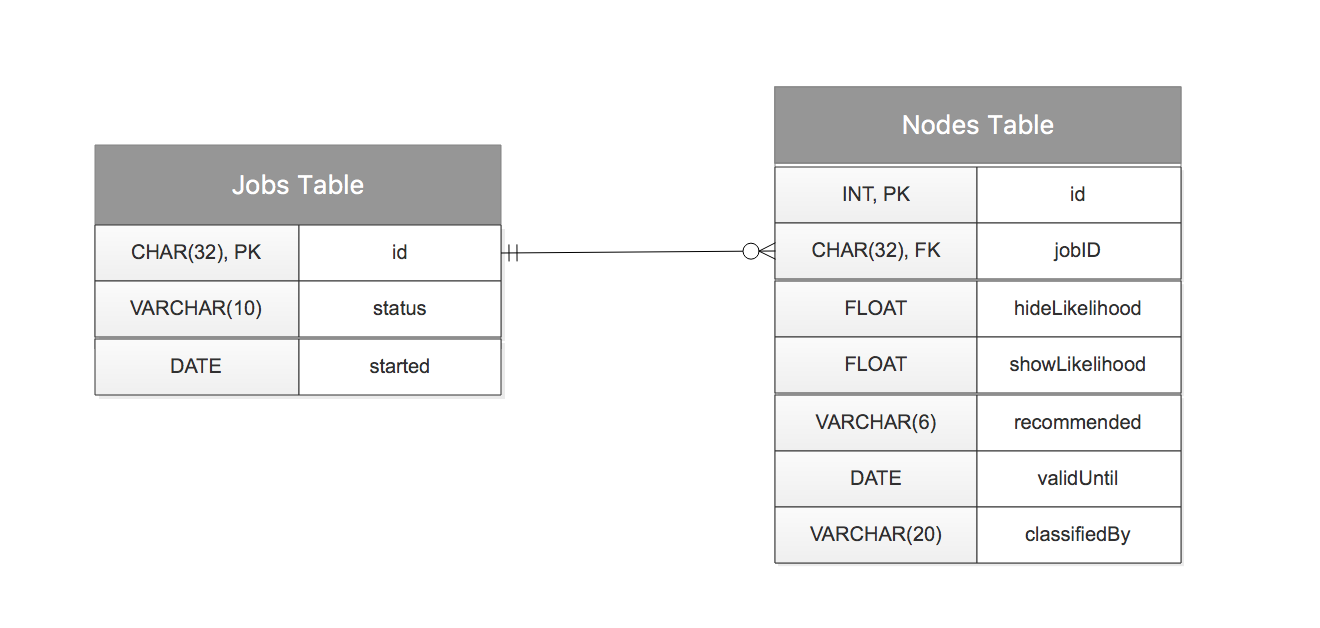
\includegraphics[width=.7\textwidth]{graphics/cache-schema}
		\caption[Cache schema]{Figure showing the relational schema used by the caching mechanism}
		\label{Fig: impl/REST/cache/relational}
	\end{figure}
	By default, every cache entry is invalidated 24 hours after the job that the node is associated with is finished. On top of this, the API provides an entry point for forcibly clearing the cache. 
	
	\section{Modularity \& Scalability} \label{Section: impl/modularity&scalability}
	During the implementation of the API, I had two goals in mind: modularity and scalability. In order to achieve this, every section makes use of the object-oriented paradigm (as shown in Figure \ref{Fig: impl/REST/API-integrate}). This allows anyone who wants to extend the tool to do so with ease, by simply extending one class and specifying this when starting the API.  
	\begin{figure}[H]
		\centering
		\includegraphics[width=.9\textwidth]{graphics/umls/full-system-uml}
		\caption[General UML diagram]{\centering UML diagram showing the integration of API's jobs with the previous two modules(i.e. feature extractor and machine learning models).}
		\label{Fig: impl/REST/API-integrate}
	\end{figure}
	The \textbf{feature extractor} can connect to any Neo4J database that has the structure described in Section \ref{Section: prep/datastructure} and extract feature vectors for the nodes. 
	\\ \\
	Anyone can add a new machine learning model to the API, by simply extending the abstract class \textit{models.Model}. The new model can be used by the API by simply specifying it as a parameter.  
	\\ \\
	The REST-like architecture of the API allows for the server-side model to scale horizontally, by balancing the load between multiple instances of the server. The cache can then be either shared by all the instances, or have one cache for each instance. In both cases, though, the cache database can be scaled vertically by running it on a more powerful machine. 
	
	\section{Summary} \label{Section: impl/summary}
\end{document}